% N-state model chapter.
%%%%%%%%%%%%%%%%%%%%%%%%

\chapter{The N-state model or ensemble analysis} \label{ch: N-state model}
\index{N-state model|textbf}
\index{Ensemble analysis|textbf}


\begin{figure*}[h]
  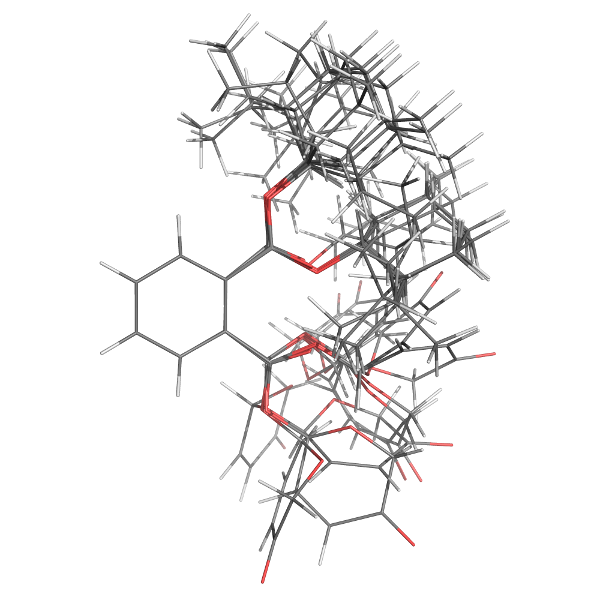
\includegraphics[width=5cm, bb=0 0 1701 1701]{graphics/misc/n_state_model/phthalic_acid_ens_600x600}
\end{figure*}


% Introduction.
%%%%%%%%%%%%%%%

\section{Introduction to the N-state model}

The modelling of motion in molecules using experimental data consists of either continuous or discrete distributions.
These can be visualised respectively as either an infinite number of states or a limited set of N states.
The N-state model analysis in relax models the molecular dynamics using an ensemble of static structures.

This analysis supports a number of data types including:
\begin{itemize}
\item Residual dipolar couplings (RDCs)\index{Residual dipolar coupling}
\item Pseudo-contact shifts (PCSs)\index{Pseudo-contact shifts}
\item NOEs\index{NOE}
\end{itemize}

The main idea is to evaluate the quality of a fixed ensemble of structures.
relax will not perform structural optimisations.
The evaluation includes:
\begin{itemize}
\item Alignment tensor optimisation for the RDCs and PCSs.
\item Optional optimisation of the position of the paramagnetic centre for the PCSs.
\item Calculation of NOE constraint violations.
\item Q factor calculation for the RDC, PCS, and NOE.
\end{itemize}

Note that this analysis will also handle single structures.
Hence you can use the N-state model in relax with N set to 1 to find, for example, a single alignment tensor for a single structure using RDCs, PCSs, or both together.
This is useful for comparing a ensemble to a single structure to determine if any statistically significant motions are present.

The primary references for the N-state model analysis in relax are:
\begin{itemize}
  \item \bibentry{Sun11}
  \item \bibentry{Erdelyi11}
\end{itemize}



% Data types.
%%%%%%%%%%%%%
 
\section{Experimental data support for the N-state model}

% RDCs.
\subsection{RDCs in the N-state model}

Residual dipolar couplings (RDCs)\index{Residual dipolar coupling|textbf} can be used to evaluate ensembles.  
The ensemble interconversion is assumed to be fast relative to timescale of the alignment process, hence a single tensor for all members of the ensemble will be used.
As such, precise superimposition of structures using a logical frame of reference is very important.
This can be performed in relax using the \uf{structure\ufsep{}superimpose} user function.
The RDCs can either be from external or internal alignment.


% PCSs.
\subsection{PCSs in the N-state model}

Pseudo-contact shifts (PCSs)\index{Pseudo-contact shifts|textbf} can also be used to evaluate ensembles.  
The same averaging process as described above for the RDC is assumed.
Hence correct structural superimposition is essential and one alignment tensor will be optimised for the entire ensemble.

One powerful feature of relax is that the paramagnetic centre can either be fixed or be allowed to move during optimisation.
This allows an unknown paramagnetic centre position to be found.
Or a known position to be refined to higher accuracy than that possible with most other techniques.


% NOEs.
\subsection{NOEs in the N-state model}

Another data type which can be used to evaluate dynamics ensembles is the NOE\index{NOE|textbf}.
This is not used in optimisation but rather is used to calculate NOE constraint violations.
These violations are then compared to evaluate the ensemble.
In the stereochemistry auto-analysis, these violations will also be converted to Q factors to allow direct comparison with RDC Q factors.



% Stereochemistry.
%%%%%%%%%%%%%%%%%%

\section{Determining stereochemistry in dynamic molecules}

A published application of the N-state model in relax is:
\begin{itemize}
  \item \bibentry{Sun11}
\end{itemize}

This analysis of the stereochemistry of a small molecule consists of two steps.
The first part is to determine the relative configuration.
The idea is to use NMR data (consisting of RDCs and NOEs) to find the relative configuration.
Ensembles of 10 members are created from molecular dynamics simulations (MD)\index{molecular dynamics simulation} or simulated annealing (SA)\index{simulated annealing}.
These are then ranked by the RDC Q factor and NOE violation.
By converting the NOE violation into a Q factor:
\begin{equation}
    Q_{\textrm{NOE}}^2 = \frac{U}{\sum_i \textrm{NOE}^2},
\end{equation}

where U is the quadratic flat bottom well potential, i.e.\ the NOE violation in \AA$^2$, and the denominator is the sum of all squared NOEs.
A combined Q factor is calculated as:
\begin{equation}
    Q_{\textrm{total}}^2 = Q_{\textrm{NOE}}^2 + Q_{\textrm{RDC}}^2.
\end{equation}

The second step is to distinguish enantiomers.
As NMR data is symmetric, it cannot distinguish enantiomers.
Therefore an optical technique such as \href{http://en.wikipedia.org/wiki/Optical\_rotatory\_dispersion}{optical rotatory dispersion} can be used.
For molecules experiencing large amounts of motion, sampling all possible conformations, calculating the expected dispersion properties, and calculating an averaged dispersion curve is not feasible.
The idea is therefore to combine NMR and ORD by taking the best NMR ensembles from step one to use for ORD spectral prediction.


% Auto-analysis.
%~~~~~~~~~~~~~~~

\subsection{Stereochemistry -- the auto-analysis}


Step one of the N-state model is implemented as an auto-analysis.
This is located in the module \module{auto\_analysis\pysep{}stereochem\_analysis} (see \url{http://www.nmr-relax.com/api/3.1/auto_analyses.stereochem_analysis-module.html}).
The auto-analysis is accessed via the \module{Stereochem\_\linebreak[0]analysis} class, the details of which can be seen at \url{http://www.nmr-relax.com/api/3.1/auto_analyses.stereochem_analysis.Stereochem_analysis-class.html}.


% The sample script.
%~~~~~~~~~~~~~~~~~~~

\subsection{Stereochemistry -- the sample script}

The following script was used for the analysis in \citet{Sun11}.
It is used to complete the first step of the analysis, the determination of relative configuration, and for the generation of ensembles for the second step of the analysis.


\begin{lstlisting}
"""Script for the determination of relative stereochemistry.

The analysis is preformed by using multiple ensembles of structures, randomly sampled from a given set of structures.  The discrimination is performed by comparing the sets of ensembles using NOE violations and RDC Q factors.

This script is split into multiple stages:

    1.  The random sampling of the snapshots to generate the N ensembles (NUM_ENS, usually 10,000 to 100,000) of M members (NUM_MODELS, usually ~10).  The original snapshot files are expected to be named the SNAPSHOT_DIR + CONFIG + a number from SNAPSHOT_MIN to SNAPSHOT_MAX + ".pdb", e.g. "snapshots/R647.pdb".  The ensembles will be placed into the "ensembles" directory.

    2.  The NOE violation analysis.

    3.  The superimposition of ensembles.  For each ensemble, Molmol is used for superimposition using the fit to first algorithm.  The superimposed ensembles will be placed into the "ensembles_superimposed" directory.  This stage is not necessary for the NOE analysis.

    4.  The RDC Q factor analysis.

    5.  Generation of Grace graphs.

    6.  Final ordering of ensembles using the combined RDC and NOE Q factors, whereby the NOE Q factor is defined as::

        Q^2 = U / sum(NOE_i^2),

    where U is the quadratic flat bottom well potential - the NOE violation in Angstrom^2. The denominator is the sum of all squared NOEs - this must be given as the value of NOE_NORM.  The combined Q is given by::

        Q_total^2 = Q_NOE^2 + Q_RDC^2.
"""

# relax module imports.
from auto_analyses.stereochem_analysis import Stereochem_analysis


# Stage of analysis (see the docstring above for the options).
STAGE = 1

# Number of ensembles.
NUM_ENS = 100000

# Ensemble size.
NUM_MODELS = 10

# Configurations.
CONFIGS = ["R", "S"]

# Snapshot directories (corresponding to CONFIGS).
SNAPSHOT_DIR = ["snapshots", "snapshots"]

# Min and max number of the snapshots (corresponding to CONFIGS).
SNAPSHOT_MIN = [0, 0]
SNAPSHOT_MAX = [76, 71]

# Pseudo-atoms.
PSEUDO = [
    ["Q7",  ["@H16", "@H17", "@H18"]],
    ["Q9",  ["@H20", "@H21", "@H22"]],
    ["Q10", ["@H23", "@H24", "@H25"]]
]

# NOE info.
NOE_FILE = "noes"
NOE_NORM = 50 * 4**2    # The NOE normalisation factor (sum of all NOEs squared).

# RDC file info.
RDC_NAME = "PAN"
RDC_FILE = "pan_rdcs"
RDC_SPIN_ID1_COL = 1
RDC_SPIN_ID2_COL = 2
RDC_DATA_COL = 2
RDC_ERROR_COL = None

# Bond length.
BOND_LENGTH = 1.117 * 1e-10

# Log file output (only for certain stages).
LOG = True

# Number of buckets for the distribution plots.
BUCKET_NUM = 200

# Distribution plot limits.
LOWER_LIM_NOE = 0.0
UPPER_LIM_NOE = 600.0
LOWER_LIM_RDC = 0.0
UPPER_LIM_RDC = 1.0


# Set up and code execution.
analysis = Stereochem_analysis(
    stage=STAGE,
    num_ens=NUM_ENS,
    num_models=NUM_MODELS,
    configs=CONFIGS,
    snapshot_dir=SNAPSHOT_DIR,
    snapshot_min=SNAPSHOT_MIN,
    snapshot_max=SNAPSHOT_MAX,
    pseudo=PSEUDO,
    noe_file=NOE_FILE,
    noe_norm=NOE_NORM,
    rdc_name=RDC_NAME,
    rdc_file=RDC_FILE,
    rdc_spin_id1_col=RDC_SPIN_ID1_COL,
    rdc_spin_id2_col=RDC_SPIN_ID2_COL,
    rdc_data_col=RDC_DATA_COL,
    rdc_error_col=RDC_ERROR_COL,
    bond_length=BOND_LENGTH,
    log=LOG,
    bucket_num=BUCKET_NUM,
    lower_lim_noe=LOWER_LIM_NOE,
    upper_lim_noe=UPPER_LIM_NOE,
    lower_lim_rdc=LOWER_LIM_RDC,
    upper_lim_rdc=UPPER_LIM_RDC
)
analysis.run()
\end{lstlisting}
